\documentclass[11pt]{article}
\usepackage[a4paper,margin=0.9in]{geometry}
\usepackage{amsmath,amssymb,amsthm,mathtools,bm}
\usepackage{graphicx}
\graphicspath{{figures/}}
\usepackage{booktabs}
\usepackage{subcaption}
\usepackage{enumitem}
\usepackage{microtype}
\usepackage{hyperref}
\usepackage{xcolor}
\usepackage{siunitx}
\usepackage{array}
\usepackage{longtable}
\usepackage{lmodern}
\usepackage{float}
\hypersetup{colorlinks=true,linkcolor=blue!50!black,citecolor=blue!50!black,urlcolor=blue!50!black}
\setlength{\parindent}{0pt}
\setlength{\parskip}{0.55em}
\newtheorem{theorem}{Theorem}[section]
\newtheorem{proposition}[theorem]{Proposition}
\newtheorem{lemma}[theorem]{Lemma}
\newtheorem{remark}[theorem]{Remark}
\newcommand{\Ncdf}{\mathcal{N}}
\newcommand{\R}{\mathbb{R}}
\newcommand{\eps}{\varepsilon}
\newcommand{\dd}{\mathrm{d}}
\newcommand{\Vega}{\mathcal{V}}

\title{\textbf{Volatility surfaces and log-normal mixture: Crafting the perfect\\
arbitrage-free calibration}\\[0.35em]\large Revised version}
\author{Abdelmalek El Alaoui}
\date{September 2026}

\begin{document}
\maketitle

\begin{abstract}
Building an arbitrage-free volatility smile that fits market quotes perfectly is a non-trivial problem. A possible approach is to assume a positive market risk-neutral distribution from which the volatility smile can be implied. A mixture of log-normal densities is a fundamental example that provides closed-form formulas for European option prices, the density, and local volatility. In this paper, we prove that any discrete arbitrage-free smile can be reproduced by a log-normal mixture distribution.

This document is a revised version of the original article \cite{elalaoui2023}. The theoretical content, notation, and proof strategy are intentionally preserved, apart from the correction of the compact interval used in the calendar-spread proof from $[0,k_{\max}]$ to $[\eta,k_{\max}]$, with $\eta>0$. The numerical section is extended with additional FX and equity examples, a comparison of two kernel-width floors, and a separate study of equity right-wing extrapolation. The bibliography is also updated to acknowledge related exact-calibration results that were not known to the author at the time of the first version.
\end{abstract}

\section{Introduction}
The Black--Scholes model \cite{blackscholes} is a cornerstone of European option pricing. It assumes constant volatility and normally distributed returns. Despite its simplicity, the model embeds the basic arbitrage-free structure and remains a fundamental tool for model design. In practice, however, the assumption of constant volatility is not realistic: observed implied volatilities vary with strike and maturity, forming a discrete grid of quotes known as the volatility smile. Many attempts to connect these quotes with a continuous arbitrage-free volatility curve do not always produce a satisfactory fit. This problem is particularly visible when the market smile has an unusual shape. For instance, the smile of a pegged currency may display a very strong skew together with a small at-the-money volatility, and a naive interpolation may easily violate arbitrage-free conditions.

Various parametric forms of the implied-volatility surface have been proposed in the literature. While some models prioritize robustness and precision, others focus more directly on the absence of arbitrage. Gatheral and Jacquier \cite{gatheraljacquier}, for example, study a parametric total-variance form designed to preserve static-arbitrage conditions. Such parametrizations are useful but cannot always capture the whole market smile accurately.

Another approach is to use a parametric representation of the market density. Starting from a positive density naturally preserves the convexity of call prices. A fundamental example was studied by Brigo and Mercurio \cite{brigo2000,brigo2002,mixedup}, where the market density is represented as a mixture of log-normal densities. This representation yields closed-form formulas for option prices, density, and local volatility, although the basic formulation alone does not guarantee a perfect fit of every market quote. Bloch and Coello \cite{blochcoello} propose a related representation with improved fitting properties but a more involved calibration.

Andreasen and Huge \cite{andreasenhuge} introduce another approach based on a local-volatility risk-neutral model defined through a one-step differential equation on a given time grid. The local volatility is taken piecewise constant in strike and is solved through least-squares minimization. The method depends on the discretization choice, and several enhancements have subsequently been discussed in the literature.

Kahal\'e \cite{kahale} proposes an arbitrage-free construction of the call-price surface by joining convex call functions over the strike grid. The parameters are solved numerically to fit the market quotes, although convergence in the smooth $C^2$ case is not established in that construction. Blacque-Florentin and Missaoui \cite{blacqueflorentin} develop a non-parametric method based on $\ell^1$ recovery; its non-parametric character does not by itself produce a smooth surface unless a smoothness penalty is added. De March and Henry-Labord\`ere \cite{demarch} formulate the calibration as the solution of a probability measure that minimizes a distance to the market, using an extension of Sinkhorn's algorithm. The method preserves arbitrage-free features but depends on the choice of a prior or reference measure. Cousot \cite{cousot2007} also studies the relation between finite option-price sets, absence of arbitrage, and exact calibration. At the time of the first version of this article, the author was not aware of Cousot's result; the present revision adds this reference to acknowledge that earlier related work. The linear interpolation used below is, however, a different object from Cousot's construction: here it is the direct strike-wise chordal interpolation of a single-maturity normalized call smile, used as an upper envelope and as the zero-width limit of the mixture.

The purpose of this paper is to design a log-normal mixture representation that can match any discrete arbitrage-free smile. We first give an intuition for the model from a degenerate case, then prove, for a given maturity, the existence of a smooth log-normal mixture that matches a discrete arbitrage-free smile perfectly. Finally, we present a straightforward calibration algorithm and numerical examples.

\textbf{Revision note.} This revised version deliberately preserves the mathematical content and organization of the original article \cite{elalaoui2023}. The calendar-spread argument is corrected on the compact interval $[\eta,k_{\max}]$ in Section~\ref{sec:calendar}. The numerical section is extended with EUR/USD, USD/HKD, dense equity examples, a sensitivity study for $\eta=10\%$ and $\eta=2\%$, and a separate equity-wing extrapolation study. The reference to Cousot \cite{cousot2007} is added because this related earlier result was not known to the author when the first version was written.

\section{Model design}
\subsection{Notations}
Fix a maturity $T$ and let $F_T$ denote the forward. We use normalized moneyness
\[
    k=\frac{K}{F_T}
\]
and total volatility $v=\sigma\sqrt{T}$. The normalized, undiscounted Black--Scholes call price is
\begin{equation}
C(k,v)=\Ncdf\!\left(-\frac{\log k}{v}+\frac{v}{2}\right)
-k\,\Ncdf\!\left(-\frac{\log k}{v}-\frac{v}{2}\right).
\label{eq:bs}
\end{equation}
For a shifted log-normal component centered at $k_j$ we write
\begin{equation}
C(k_j,k,v)
=k_j\Ncdf\!\left(-\frac{\log(k/k_j)}{v}+\frac{v}{2}\right)
-k\Ncdf\!\left(-\frac{\log(k/k_j)}{v}-\frac{v}{2}\right).
\label{eq:shifted-bs}
\end{equation}
At zero width,
\begin{equation}
C(k_j,k,0)=(k_j-k)^+.
\label{eq:zero-width}
\end{equation}

Let
\[
0<k_1<\cdots<k_N,
\qquad c_i=C(k_i,v_i),
\]
and set $(k_0^{\rm ref},c_0^{\rm ref})=(0,1)$ only for the purpose of defining the first market slope. Put
\[
\Delta_i=\frac{c_i-c_{i-1}}{k_i-k_{i-1}},\qquad i=1,\ldots,N,
\qquad \Delta_{N+1}=0.
\]
The discrete smile is free of static butterfly arbitrage when the call prices satisfy the normalized bounds and the slopes are non-decreasing:
\begin{equation}
-1\le \Delta_1\le\Delta_2\le\cdots\le\Delta_{N+1}=0,
\qquad
(1-k_i)^+\le c_i<1.
\label{eq:discrete-arb}
\end{equation}
A continuous normalized call function $c$ is statically arbitrage-free if it is decreasing, convex, and satisfies
\[
(1-k)^+\le c(k)\le1.
\]

\subsection{Upper bound interpolation}
As in the original article, define the piecewise-linear call interpolation by
\begin{equation}
 c_L(k)=
 \begin{cases}
 c_i+\Delta_{i+1}(k-k_i), & k_i\le k\le k_{i+1},\quad i=0,\ldots,N-1,\\[1mm]
 c_N, & k>k_N,
 \end{cases}
 \label{eq:original-linear-interpolation}
\end{equation}
where $(k_0,c_0)=(0,1)$ for this interpolation. This is the strike-wise chordal interpolation introduced in the previous version of this article. It should not be confused with the model construction studied by Cousot \cite{cousot2007}: the present $c_L$ is used as an elementary upper envelope of one maturity slice and as the discrete zero-width prototype of the mixture.

\begin{proposition}[Linear upper envelope]\label{prop:upper}
If the discrete quotes satisfy \eqref{eq:discrete-arb}, then $c_L$ is statically arbitrage-free. Moreover, if $f$ is any convex call function satisfying $f(k_i)=c_i$, then $f(k)\le c_L(k)$ between consecutive market strikes.
\end{proposition}

\begin{proof}
On each interval $[k_i,k_{i+1}]$, the slope of $c_L$ equals $\Delta_{i+1}$. Since the sequence $(\Delta_i)$ is increasing and non-positive, $c_L$ is convex and decreasing. The call bounds follow by linear interpolation of the endpoint inequalities; on the right, $c_L(k)=c_N\ge(1-k_N)^+\ge(1-k)^+$. Finally, a convex function lies below the chord joining any two points of its graph, hence $f\le c_L$ on each market interval.
\end{proof}

The distributional second derivative of $c_L$ is a Dirac comb. At an interior knot $k_i$ its mass is the slope jump
\begin{equation}
w_i^L=\Delta_{i+1}-\Delta_i\ge0.
\label{eq:dirac-weight}
\end{equation}
This is the discrete prototype of the risk-neutral density.

\paragraph{Lower admissible bound.}
The upper envelope is complemented by a lower one. Define
\begin{equation}
\phi(k)=
\begin{cases}
\max\{c_1+\Delta_2(k-k_1),\,1-k\}, & 0\le k\le k_1,\\[1.5mm]
\max\{c_i+\Delta_i(k-k_i),\,c_{i+1}+\Delta_{i+2}(k-k_{i+1})\},
& k_i\le k\le k_{i+1},\\[1.5mm]
\max\{c_N+\Delta_N(k-k_N),\,0\}, & k>k_N.
\end{cases}
\label{eq:phi}
\end{equation}

\begin{lemma}[Admissible interval]\label{lem:admissible}
Let $c\in C^1$ be statically arbitrage-free and satisfy $c(k_i)=c_i$. Then
\[
\phi(k)\le c(k)\le c_L(k),\qquad k\ge0.
\]
Conversely, if a new quote $(k,c_k)$ satisfies
\[
\phi(k)\le c_k\le c_L(k),
\]
then the enlarged discrete quote set remains arbitrage-free.
\end{lemma}

\begin{proof}
The upper bound is Proposition~\ref{prop:upper}. For the lower bound, convexity implies that the derivative at $k_i$ cannot lie below the incoming discrete slope $\Delta_i$ and cannot lie above the outgoing comparison slope $\Delta_{i+2}$ at $k_{i+1}$. Supporting-line inequalities therefore give
\[
c(k)\ge c_i+\Delta_i(k-k_i),\qquad
c(k)\ge c_{i+1}+\Delta_{i+2}(k-k_{i+1})
\]
on $[k_i,k_{i+1}]$. The endpoint intervals follow similarly, together with the intrinsic lower bounds $1-k$ and $0$.

For the converse, inserting $(k,c_k)$ replaces one old slope by two new slopes. The inequalities $c_k\ge\phi(k)$ give the required lower and upper bounds on these two new slopes, while $c_k\le c_L(k)$ gives their correct ordering relative to the chord slope. Thus the complete slope sequence remains non-decreasing. The call bounds also follow from $\phi(k)\ge(1-k)^+$ and $c_L(k)\le1$.
\end{proof}

\subsection{A Black--Scholes Kernel}
The discrete second derivative of the piecewise-linear interpolation is a combination of Dirac masses. A natural smooth regularization is obtained by replacing every Dirac mass centered at $k_i$ by a log-normal kernel. For a center $k_i$ and width $\sigma_i>0$, define
\begin{equation}
f(k_i,k,\sigma_i)=\frac{1}{k\sigma_i\sqrt{2\pi}}
\exp\left[-\frac{1}{2\sigma_i^2}\left(\log\frac{k}{k_i}+\frac{\sigma_i^2}{2}\right)^2\right].
\end{equation}
The corresponding call contribution is the shifted Black--Scholes function $C(k_i,k,\sigma_i)$ defined above. A positive weighted sum of these kernels therefore generates the call function
\begin{equation}
c(\widetilde{\sigma},k)=\sum_j w_j C(k_j,k,\sigma_j),
\end{equation}
and a positive smooth density. This is the basic kernel used throughout the rest of the article.

\section{Smooth solution and calibration}\label{sec:exactproof}
\subsection{Existence of a perfect fit}
Introduce two artificial quotes
\[
(k_0,c_0),\qquad (k_{N+1},c_{N+1}),
\]
with
\[
0<k_0<k_1<\cdots<k_N<k_{N+1}.
\]
Define the extended slopes
\[
\widetilde\Delta_0=-1,
\qquad
\widetilde\Delta_i=\frac{c_i-c_{i-1}}{k_i-k_{i-1}},\quad i=1,\ldots,N+1,
\qquad
\widetilde\Delta_{N+2}=0,
\]
and the slope-jump masses
\begin{equation}
w_j=\widetilde\Delta_{j+1}-\widetilde\Delta_j,
\qquad j=0,\ldots,N+1.
\label{eq:extendedweights}
\end{equation}
Arbitrage-free completion guarantees $w_j\ge0$.

\begin{lemma}[Zeroth and first moments]\label{lem:moments}
For the extended slope-jump masses,
\begin{equation}
\sum_{j=0}^{N+1}w_j=1
\label{eq:massone}
\end{equation}
and
\begin{equation}
\sum_{j=0}^{N+1}w_jk_j=1+p_0-c_{N+1},
\qquad p_0:=c_0+k_0-1.
\label{eq:firstmoment}
\end{equation}
Hence, if $p_0=c_{N+1}$, the weights define a probability law with normalized forward equal to one.
\end{lemma}

\begin{proof}
The mass identity telescopes immediately:
\[
\sum_{j=0}^{N+1}w_j
=\widetilde\Delta_{N+2}-\widetilde\Delta_0=1.
\]
For the first moment,
\begin{align*}
\sum_{j=0}^{N+1}k_jw_j
&=\sum_{j=0}^{N+1}k_j(\widetilde\Delta_{j+1}-\widetilde\Delta_j)\\
&=-\widetilde\Delta_0k_0
+\sum_{j=1}^{N+1}\widetilde\Delta_j(k_{j-1}-k_j)\\
&=k_0+\sum_{j=1}^{N+1}(c_{j-1}-c_j)\\
&=k_0+c_0-c_{N+1}=1+p_0-c_{N+1}.
\end{align*}
\end{proof}

\begin{lemma}[Existence of compatible boundary quotes]\label{lem:boundary}
There exist continuous admissible boundary selections $l$ on $[0,k_1]$ and $r$ on $[k_N,\infty)$ such that, for all sufficiently large $R$, one can find $k_0\in(0,k_1)$ with
\[
c_0=l(k_0),\qquad k_{N+1}=R,\qquad c_{N+1}=r(R),
\]
and
\begin{equation}
k_0+c_0-c_{N+1}=1.
\label{eq:boundarymoment}
\end{equation}
Moreover, $c_{N+1}\downarrow0$ and $k_0\downarrow0$ as $R\to\infty$.
\end{lemma}

\begin{proof}
Choose $l(k)$ continuously between the lower and upper admissible envelopes $\phi(k)$ and $c_L(k)$ on $[0,k_1]$, with $l(0)=1$ and $l(k_1)=c_1$. For example, a fixed convex combination of $\phi$ and $c_L$ suffices. Define
\[
h(k)=k+l(k)-1.
\]
Then $h$ is continuous, $h(0)=0$, and $h(k_1)=p_1:=c_1+k_1-1>0$.

On the right, choose a continuous function $r(R)$ satisfying
\[
\phi(R)\le r(R)\le c_L(R)=c_N,
\qquad r(R)\downarrow0.
\]
One may take a convex combination of $c_N$ and $\phi(R)$ with a coefficient tending to zero. By Lemma~\ref{lem:admissible}, each selected boundary quote is arbitrage-free. For $R$ sufficiently large, $0<r(R)<p_1$. The intermediate value theorem then gives $k_0\in(0,k_1)$ such that
\[
h(k_0)=r(R),
\]
which is exactly \eqref{eq:boundarymoment}. Since $r(R)\to0$ and $h(k)>0$ for $k>0$ sufficiently close to the origin, the selected $k_0$ also tends to zero.
\end{proof}

From now on write
\[
\eps:=c_{N+1}=p_0>0.
\]
Then Lemma~\ref{lem:moments} gives both moment constraints exactly.

\paragraph{The zero-width prototype.}
For a width vector $\bm\sigma=(\sigma_0,\ldots,\sigma_{N+1})$, define
\begin{equation}
g(k;\bm\sigma)=\sum_{j=0}^{N+1}w_jC(k_j,k,\sigma_j).
\label{eq:gmixture}
\end{equation}

\begin{lemma}[Zero-width displacement]\label{lem:zero}
For every extended knot $k_i$, $i=1,\ldots,N+1$,
\begin{equation}
g(k_i;\bm0)=c_i-\eps.
\label{eq:zerodisplacement}
\end{equation}
\end{lemma}

\begin{proof}
Using \eqref{eq:zero-width},
\[
g(k_i;\bm0)=\sum_{j=i}^{N+1}w_j(k_j-k_i).
\]
Substituting $w_j=\widetilde\Delta_{j+1}-\widetilde\Delta_j$ and summing by parts gives
\[
g(k_i;\bm0)
=\sum_{j=i+1}^{N+1}(c_{j-1}-c_j)
=c_i-c_{N+1}=c_i-\eps.
\]
The same identity can be interpreted geometrically: the zero-width mixture equals the completed piecewise-linear call function translated downward by the common boundary level $\eps$.
\end{proof}

Thus every market equation can be rewritten as the same smoothing increment:
\begin{equation}
\sum_{j=0}^{N+1}w_j
\bigl[C(k_j,k_i,\sigma_j)-C(k_j,k_i,0)\bigr]
=\eps,
\qquad i=1,\ldots,N+1.
\label{eq:system}
\end{equation}

\paragraph{First-order localization.}
Let
\[
\Vega(k_j,k,s):=\frac{\partial}{\partial s}C(k_j,k,s).
\]
For $s>0$,
\begin{equation}
\Vega(k_j,k,s)
=\frac{k_j}{\sqrt{2\pi}}
\exp\!\left[-\frac12\left(\frac{s}{2}-\frac{\log(k/k_j)}{s}\right)^2\right].
\label{eq:vega}
\end{equation}
Hence
\begin{equation}
\Vega(k_i,k_i,0)=\frac{k_i}{\sqrt{2\pi}},
\qquad
\Vega(k_j,k_i,0)=0\quad(j\ne i),
\label{eq:vegazero}
\end{equation}
where the off-diagonal value is understood by continuity.

Taylor's theorem gives, for suitable $\xi_{ij}\in(0,\sigma_j)$,
\begin{align}
w_i\bigl[C(k_i,k_i,\sigma_i)-C(k_i,k_i,0)\bigr]
&=w_i\Vega(k_i,k_i,0)\sigma_i
+\frac12w_i\partial_s\Vega(k_i,k_i,\xi_{ii})\sigma_i^2,
\label{eq:taylor-diag}\\
w_j\bigl[C(k_j,k_i,\sigma_j)-C(k_j,k_i,0)\bigr]
&=\frac12w_j\partial_s\Vega(k_j,k_i,\xi_{ij})\sigma_j^2,
\quad j\ne i.
\label{eq:taylor-off}
\end{align}
Therefore the system is diagonally dominant to first order. The first-order solution is
\begin{equation}
\sigma_i^{(1)}
=\frac{\eps}{w_i\Vega(k_i,k_i,0)}
=\frac{\eps\sqrt{2\pi}}{w_i k_i}.
\label{eq:firstorder}
\end{equation}
If an interior slope jump is exactly zero, its zero-mass component is simply removed before applying the argument; the collinear case then follows by continuity.

\paragraph{Uniform control of the quadratic terms.}
The derivative of vega can be written explicitly. With
\[
L_{ij}=\log\frac{k_i}{k_j},
\]
we have
\begin{equation}
\partial_s\Vega(k_j,k_i,s)
=\frac{k_j}{\sqrt{2\pi}}
\frac{L_{ij}^2-\frac14s^4}{s^3}
\exp\!\left[-\frac12\left(\frac{s}{2}-\frac{L_{ij}}{s}\right)^2\right].
\label{eq:vomma}
\end{equation}

\begin{lemma}[Off-diagonal bound]\label{lem:vomma-bound}
Fix $\nu>0$ and $\mu>0$. There exist constants $M_\mu>0$ and $R_0>k_N$, depending only on the original market quotes and on $(\nu,\mu)$, such that for every sufficiently large right artificial strike $R=k_{N+1}\ge R_0$ and every $s\in[0,\nu]$:
\begin{enumerate}[label=(\roman*)]
\item for distinct non-extreme centers, $|\partial_s\Vega(k_j,k_i,s)|\le M_\mu k_j^2$;
\item for the right artificial center, $|\partial_s\Vega(R,k_i,s)|\le M_\mu R$;
\item the analogous bounds involving $k_0$ hold uniformly as $k_0\downarrow0$.
\end{enumerate}
\end{lemma}

\begin{proof}
For fixed distinct market centers, \eqref{eq:vomma} extends continuously to $s=0$ with value zero and tends to zero as $s\to\infty$; it is therefore bounded on $[0,\nu]$. For the moving boundary centers, write the exponential factor in terms of $L=L_{ij}$. If $|L|>\mu$, the polynomial prefactor in \eqref{eq:vomma} is dominated by the Gaussian term
\[
\exp\!\left[-\frac{L^2}{2s^2}+O(|L|)\right],
\]
uniformly for $s\le\nu$. Consequently the rescaled functions appearing after factoring $k_i$, $k_j^2/k_i$, or $R$ have finite suprema independent of the boundary location. Since $R\to\infty$ and $k_0\to0$, the logarithmic separations from every fixed market center eventually exceed $\mu$. Taking the maximum over the finitely many remaining market pairs gives a common constant $M_\mu$.
\end{proof}

The role of Lemma~\ref{lem:vomma-bound} is to ensure that all off-diagonal terms in \eqref{eq:taylor-off} remain uniformly of order $\eps^2$, including those generated by the moving artificial boundaries.

\paragraph{Miranda--Poincar\'e argument.}
Define, for $i=1,\ldots,N+1$,
\begin{equation}
f_i(\bm\sigma)=
\sum_{j=0}^{N+1}w_j
\bigl[C(k_j,k_i,\sigma_j)-C(k_j,k_i,0)\bigr]-\eps.
\label{eq:fi}
\end{equation}
The required fit is equivalent to $f_i=0$ for all $i$.

Choose a constant
\[
A>1+\sup_{s\ge0}\left|\frac{\partial_s\Vega(k_i,k_i,s)}{\Vega(k_i,k_i,0)}\right|
\]
large enough to work simultaneously for the finitely many market centers, and define
\[
\lambda_i=1+A\sigma_i^{(1)}.
\]
Fix the left-boundary width at the positive value
\[
\sigma_0=\lambda_0\sigma_0^{(1)}
\]
and consider the box
\begin{equation}
\mathcal K=\prod_{i=1}^{N+1}[0,\lambda_i\sigma_i^{(1)}].
\label{eq:box}
\end{equation}

\begin{lemma}[Sign on the upper faces]\label{lem:upperface}
For $\eps$ sufficiently small,
\[
f_i(\sigma_1,\ldots,\sigma_{i-1},\lambda_i\sigma_i^{(1)},\sigma_{i+1},\ldots,\sigma_{N+1})\ge0
\]
for every point of the $i$th upper face of $\mathcal K$.
\end{lemma}

\begin{proof}
Each shifted Black--Scholes call is increasing in its width. Hence, on the upper face, $f_i$ is minimized when all other variable widths are zero. Using \eqref{eq:taylor-diag}, the diagonal excess above its first-order value equals
\[
w_i\Vega(k_i,k_i,0)(\lambda_i-1)\sigma_i^{(1)}
+O((\sigma_i^{(1)})^2).
\]
Because $(\lambda_i-1)=A\sigma_i^{(1)}$, the leading positive coefficient can be chosen to dominate the uniformly bounded quadratic remainder. Since $\sigma_i^{(1)}=O(\eps)$, the inequality holds for sufficiently small $\eps$.
\end{proof}

\begin{lemma}[Sign on the lower faces]\label{lem:lowerface}
For $\eps$ sufficiently small,
\[
f_i(\sigma_1,\ldots,\sigma_{i-1},0,\sigma_{i+1},\ldots,\sigma_{N+1})\le0
\]
for every point of the $i$th lower face of $\mathcal K$.
\end{lemma}

\begin{proof}
When $\sigma_i=0$, the diagonal first-order contribution is absent. Every remaining contribution is off-diagonal and therefore quadratic by \eqref{eq:taylor-off}. On the box \eqref{eq:box}, each width is $O(\eps/(w_jk_j))$. Lemma~\ref{lem:vomma-bound}, together with the boundary asymptotics $R w_{N+1}\to c_N$ and positivity of the non-zero market masses, gives a constant $B$ independent of sufficiently small $\eps$ such that
\[
\sum_{j\ne i}
\left|w_j\bigl[C(k_j,k_i,\sigma_j)-C(k_j,k_i,0)\bigr]\right|
\le B\eps^2.
\]
Thus
\[
f_i\le B\eps^2-\eps\le0
\]
for $\eps<1/B$.
\end{proof}

\begin{theorem}[Exact smooth representation]\label{thm:exact}
Let $(k_i,c_i)_{1\le i\le N}$ be a discrete arbitrage-free smile. Then there exist arbitrage-free boundary quotes and strictly positive kernel widths such that
\begin{equation}
c_i=\sum_{j=0}^{N+1}w_jC(k_j,k_i,\sigma_j),
\qquad i=1,\ldots,N,
\label{eq:exactfit}
\end{equation}
with
\[
\sum_{j=0}^{N+1}w_j=1,
\qquad
\sum_{j=0}^{N+1}w_jk_j=1.
\]
Consequently, the fitted call function is smooth and free of static strike arbitrage. Moreover,
\begin{equation}
\sigma_i
=\frac{\eps\sqrt{2\pi}}{w_i k_i}+O(\eps^2)
\label{eq:sigmaasymptotic}
\end{equation}
in the small-boundary regime.
\end{theorem}

\begin{proof}
By Lemmas~\ref{lem:upperface} and \ref{lem:lowerface}, the continuous mapping
\[
(f_1,\ldots,f_{N+1}):\mathcal K\to\R^{N+1}
\]
has non-positive $i$th component on the $i$th lower face and non-negative $i$th component on the corresponding upper face. The Miranda--Poincar\'e theorem therefore provides a point $\bm\sigma\in\mathcal K$ for which all $f_i$ vanish simultaneously. Equation \eqref{eq:fi} together with Lemma~\ref{lem:zero} gives exact reproduction of the completed call quotes, in particular of all genuine market quotes.

The weights are non-negative because they are slope jumps of an arbitrage-free completed call grid. Lemma~\ref{lem:moments} gives total mass one and first moment one. Hence the density
\[
d(k)=\sum_{j=0}^{N+1}w_j
\frac{1}{k\sigma_j\sqrt{2\pi}}
\exp\!\left[-\frac{(\log k-\log k_j)^2}{2\sigma_j^2}\right]
\]
is positive and has the correct moments, so its integrated call function is decreasing, convex, and normalized to the forward. Finally, the localization formula \eqref{eq:sigmaasymptotic} follows from the first-order balance \eqref{eq:firstorder} and the quadratic remainder bounds.
\end{proof}

\section{Calendar-spread arbitrage}\label{sec:calendar}
Let $0<t_1<\cdots<t_M$ be quoted maturities and let $c_L^j$ be the piecewise-linear call interpolation of the $j$th slice. If two adjacent fitted slices $c^j$ and $c^{j+1}$ are ordered in call price, an interpolation in time of the form
\begin{equation}
c(k,t)=\theta(t)c^{j+1}(k)+[1-\theta(t)]c^j(k),
\qquad t\in[t_j,t_{j+1}],
\label{eq:timeinterp}
\end{equation}
with $\theta$ increasing from $0$ to $1$, preserves convexity and monotonicity in strike. Calendar-spread arbitrage is excluded when
\begin{equation}
c^{j+1}(k)>c^j(k).
\label{eq:calendarcondition}
\end{equation}

The earlier version \cite{elalaoui2023} stated the compact convergence argument on $[0,k_{\max}]$. The correct form for the vega estimate used below is on a compact interval bounded away from the singular endpoint $k=0$.

\begin{lemma}[Uniform convergence on a positive compact interval]\label{lem:calendaruniform}
Fix $\eta>0$ and $k_{\max}>k_N$. For each maturity $t_j$, let
\[
c^j_{R}(k)=c^j(\bm\sigma^j_R,k)
\]
be the fitted mixture corresponding to a right artificial strike $R$ and boundary level $\eps_R\downarrow0$. Then
\[
\sup_{k\in[\eta,k_{\max}]}
|c_R^j(k)-c_L^j(k)|\longrightarrow0
\qquad (R\to\infty).
\]
\end{lemma}

\begin{proof}
Write
\[
|c_R^j(k)-c_L^j(k)|
\le
|c_R^j(k)-c_R^j(k;\bm0)|
+
|c_R^j(k;\bm0)-c_L^j(k)|.
\]
The second term is the zero-width completion error. On the observed strike interval it is bounded by the artificial level $\eps_R$. On the bounded right extension, the rightmost intrinsic-value term converges uniformly to the flat extrapolation because $R$ tends to infinity while $Rw_{N+1}$ remains bounded and converges to the terminal call level. The analogous left-boundary error vanishes with $k_0$ and $\eps_R$. Hence the zero-width term converges uniformly to zero.

For the smoothing term, the mean-value theorem gives
\[
|c_R^j(k)-c_R^j(k;\bm0)|
\le
\|\bm\sigma_R^j\|_\infty
\sum_{\ell}w_\ell
\sup_{\substack{k\in[\eta,k_{\max}]\\0\le s\le\|\bm\sigma_R^j\|_\infty}}
\Vega(k_\ell,k,s).
\]
For fixed $R$ the sum is finite, and on $k\in[\eta,k_{\max}]$ the vega factors are continuous and uniformly bounded. The exact-fit construction yields $\|\bm\sigma_R^j\|_\infty\to0$ as $\eps_R\to0$. Therefore the smoothing term also converges uniformly to zero.
\end{proof}

\begin{theorem}[Calendar-spread preservation]\label{thm:calendar}
Assume that the piecewise-linear market slices are strictly ordered:
\[
c_L^{j+1}(k)>c_L^j(k)
\qquad
\text{for every }k\in[\eta,k_{\max}].
\]
Then the artificial boundary levels can be chosen sufficiently small so that the corresponding smooth mixture slices satisfy
\[
c^{j+1}(k)>c^j(k),
\qquad k\in[\eta,k_{\max}],
\]
and the time interpolation \eqref{eq:timeinterp} is free of strike and calendar-spread arbitrage on this domain.
\end{theorem}

\begin{proof}
For each pair of adjacent maturities, continuity on the compact interval gives a strictly positive gap
\[
\delta_j=
\min_{k\in[\eta,k_{\max}]}
\bigl[c_L^{j+1}(k)-c_L^j(k)\bigr]>0.
\]
By Lemma~\ref{lem:calendaruniform}, choose the boundary levels so that
\[
\sup_{k\in[\eta,k_{\max}]}|c^{j+1}(k)-c_L^{j+1}(k)|<\frac{\delta_j}{3},
\qquad
\sup_{k\in[\eta,k_{\max}]}|c^j(k)-c_L^j(k)|<\frac{\delta_j}{3}.
\]
Then, uniformly in $k$,
\begin{align*}
c^{j+1}(k)-c^j(k)
&\ge c_L^{j+1}(k)-c_L^j(k)
-|c^{j+1}(k)-c_L^{j+1}(k)|
-|c^j(k)-c_L^j(k)|\\
&>\delta_j-\frac{2\delta_j}{3}>0.
\end{align*}
Thus adjacent smooth slices remain ordered. A convex combination of two decreasing convex call functions is again decreasing and convex, and because $\theta$ is increasing the interpolated call price is increasing in maturity. This excludes strike and calendar-spread arbitrage on $[\eta,k_{\max}]$.
\end{proof}

If the time interpolation is differentiable, Dupire's local variance is
\begin{equation}
\sigma_D^2(k,t)
=\frac{\partial_t c(k,t)}{\frac12 k^2\partial_{kk}c(k,t)},
\end{equation}
and both numerator and denominator are explicit combinations of the calibrated slices.

\section{Calibration algorithm for a single maturity}\label{sec:calibration}
For a single maturity, the practical routine used in the numerical experiments is:
\begin{enumerate}[label=\arabic*)]
\item Convert market implied volatilities to normalized undiscounted calls.
\item Check the discrete call bounds, monotonicity, and convexity.
\item Add one boundary quote whenever possible. If $p_1>c_N$, solve a left boundary quote; if $c_N>p_1$, solve a right boundary quote. The selected boundary location balances the two neighboring boundary butterfly masses as far as the admissible geometry allows.
\item Build the slope-jump weights and the log-normal mixture.
\item Minimize the vega-scaled market objective
\begin{equation}
\Phi(\bm\sigma)=
\sum_{i\in\mathcal M}
\left(\frac{c(\bm\sigma,k_i)-c_i}{\Vega_i}\right)^2
+
\omega_{\rm art}
\left(\frac{c(\bm\sigma,k_{\rm art})-c_{\rm art}}{\Vega_{\rm art}}\right)^2,
\label{eq:objective}
\end{equation}
with a very small artificial-quote weight $\omega_{\rm art}=10^{-10}$.
\item Infer the continuous Black implied volatility from the fitted call function.
\end{enumerate}

To prevent nearly singular kernels, the calibration may impose the lower-width constraint already proposed in the original article,
\begin{equation}
\sigma_i\ge\eta\,\sigma_{\rm ATM}.
\label{eq:floor}
\end{equation}
The numerical results below report both $\eta=10\%$, which gives a stronger smoothing constraint, and $\eta=2\%$, which allows narrower kernels and therefore a more flexible fit. For the dense equity experiments, we additionally impose
\begin{equation}
\sigma_i\le3\,\sigma_{\rm ATM},
\label{eq:cap}
\end{equation}
which prevents a small number of extremely broad kernels from dominating the far equity tails. This cap is not used in the FX section.

\subsection{Example of calibration}\label{sec:results}
\subsubsection*{Cubic total-variance benchmark}
As a benchmark, we interpolate total implied variance
\[
w(x)=\sigma_{\rm imp}^2(x)T,
\qquad x=\log(K/F),
\]
with a natural cubic spline. This benchmark interpolates its knots exactly, but exact interpolation does not guarantee a non-negative risk-neutral density. The standard butterfly factor is
\begin{equation}
g(x)=
\left(1-\frac{xw'(x)}{2w(x)}\right)^2
-\frac{w'(x)^2}{4}\left(\frac{1}{w(x)}+\frac14\right)
+\frac12w''(x).
\label{eq:g}
\end{equation}
Negative values of $g$ correspond to negative density in the total-variance representation.

\subsubsection*{FX results: EUR/USD and USD/HKD}\label{sec:fxresults}
No equity wing control is used in this subsection: every calibrated mixture width remains constant for all strikes. The EUR/USD data are conventional five-point FX smiles. For USD/HKD we use the five-point forward-delta quotes reported by BofA Global Research on 21 May 2025 \cite{bofa2025}: 10-delta put, 25-delta put, ATM, 25-delta call, and 10-delta call. We convert delta to normalized strike using the forward-delta Black convention described, for example, in \cite{clark}.

The USD/HKD source contains four maturities. Table~\ref{tab:hkdquotes} reports the complete quoted smile rather than only the 6M example used in the previous numerical figure.

\begin{table}[H]
\centering
\caption{USD/HKD implied-volatility quotes (in percent) from BofA Global Research, 21 May 2025 \cite{bofa2025}.}
\label{tab:hkdquotes}
\small
\begin{tabular}{lrrrrr}
\toprule
Maturity & 10$\Delta$ Put & 25$\Delta$ Put & ATM & 25$\Delta$ Call & 10$\Delta$ Call \\
\midrule
1M & 4.40 & 2.40 & 1.59 & 1.86 & 3.33 \\
3M & 6.02 & 3.19 & 1.68 & 1.45 & 2.54 \\
6M & 7.43 & 3.90 & 1.85 & 1.15 & 1.51 \\
1Y & 8.30 & 4.40 & 2.15 & 1.40 & 1.83 \\
\bottomrule
\end{tabular}
\end{table}

The lower-width parameter has a visible effect only when the market requires narrow local components. EUR/USD is already fitted almost exactly for both values. The strongly skewed USD/HKD 6M and 1Y smiles are more sensitive: reducing the floor from 10\% to 2\% of ATM volatility recovers an essentially exact fit while the mixture density remains positive.

\begin{table}[H]
\centering
\caption{Flat-kernel FX calibration diagnostics for $\eta=10\%$ and $\eta=2\%$. No wing control is used.}
\label{tab:fx}
\small
\resizebox{\textwidth}{!}{%
\begin{tabular}{llrrrrr}
\toprule
Pair & Maturity & Quotes & Max IV error, 10\% (bp) & Max IV error, 2\% (bp) & Min. density, 10\% & Min. density, 2\% \\
\midrule
EUR/USD & 1W & 5 & $<0.001$ & $<0.001$ & 5.139 & 4.857 \\
EUR/USD & 6M & 5 & $<0.001$ & $<0.001$ & 1.034 & 1.034 \\
EUR/USD & 1Y & 5 & $<0.001$ & $<0.001$ & 0.628 & 0.628 \\
USD/HKD & 1M & 5 & 0.003 & $<0.001$ & 0.651 & 0.626 \\
USD/HKD & 3M & 5 & 0.002 & $<0.001$ & 0.263 & 0.221 \\
USD/HKD & 6M & 5 & 5.530 & $<0.001$ & 0.098 & 0.177 \\
USD/HKD & 1Y & 5 & 4.782 & $<0.001$ & 0.064 & 0.115 \\
\bottomrule
\end{tabular}%
}
\end{table}

\begin{figure}[H]
\centering
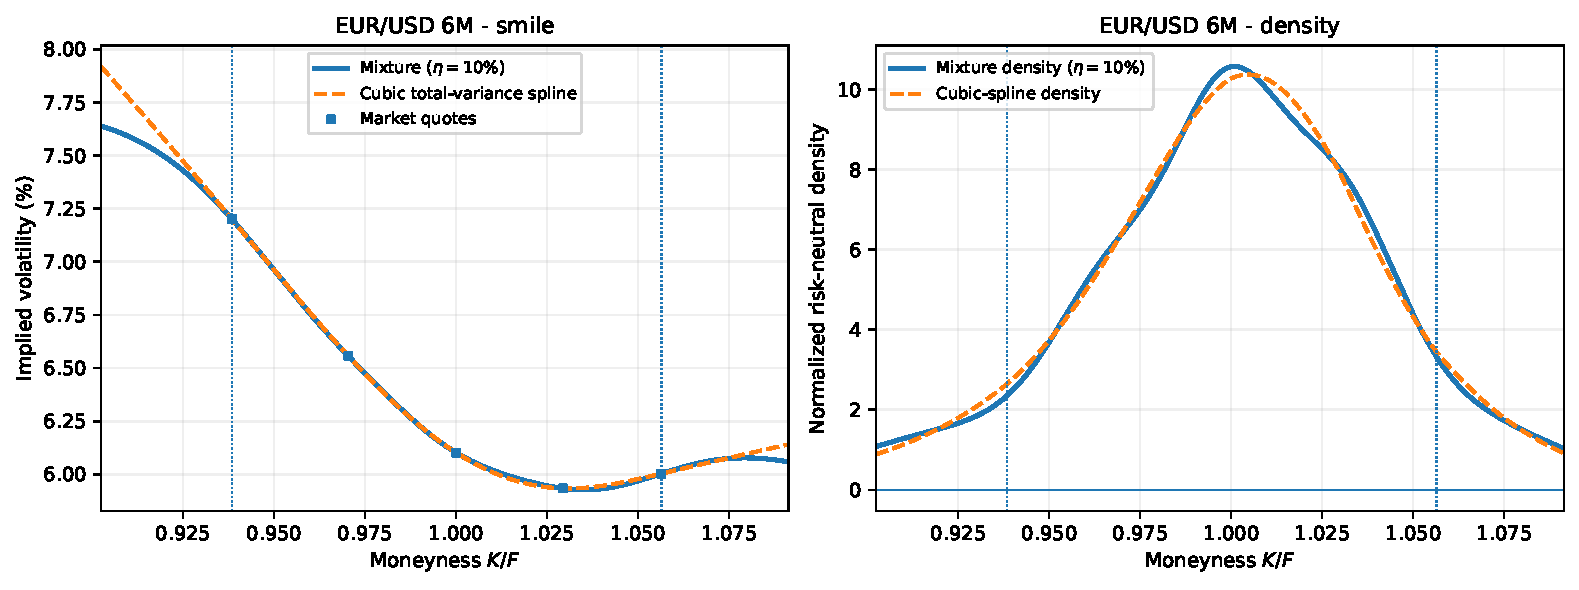
\includegraphics[width=0.98\textwidth]{fx_eurusd_6mo.pdf}
\caption{EUR/USD 6M with the 10\% floor. The log-normal mixture uses constant kernel widths on both wings; the plotting window extends beyond the observed five-point smile. Small square markers denote market quotes.}
\label{fig:eurusd6m}
\end{figure}

\begin{figure}[H]
\centering
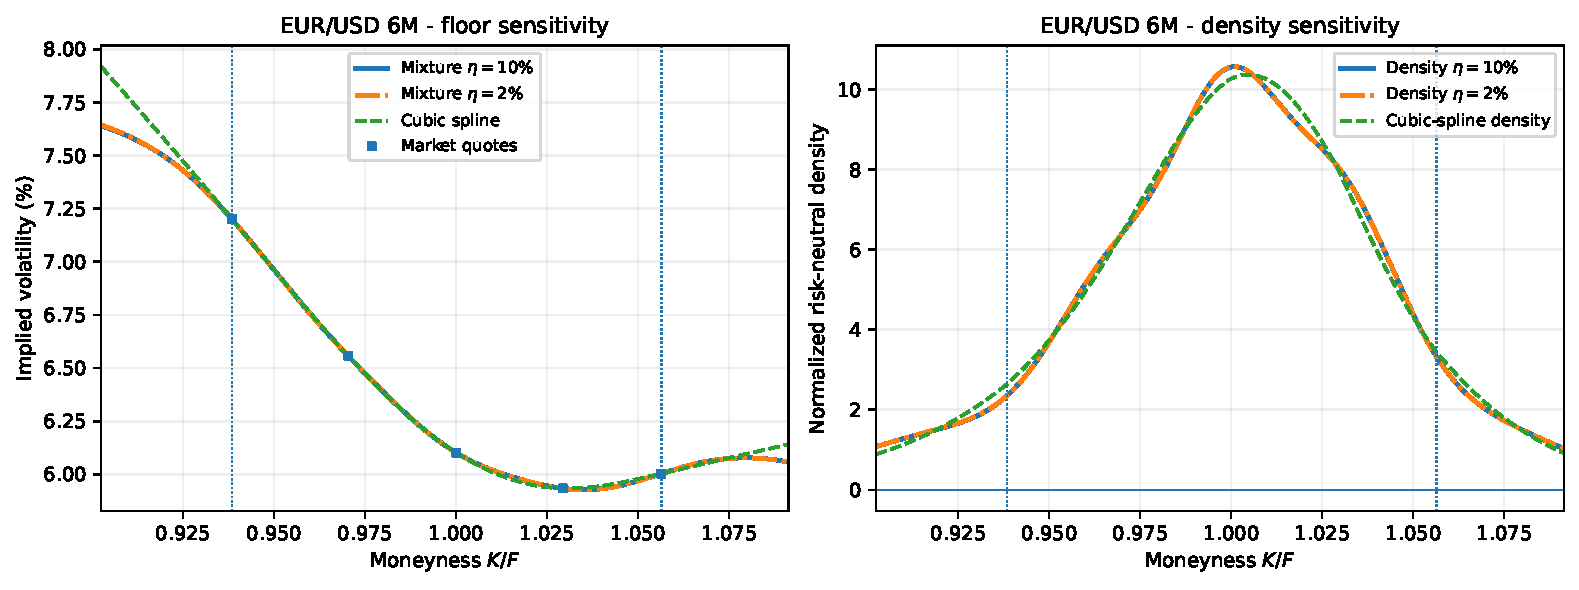
\includegraphics[width=0.98\textwidth]{fx_eurusd_eta_compare.pdf}
\caption{EUR/USD 6M sensitivity to the kernel floor. Both $\eta=10\%$ and $\eta=2\%$ reproduce the five market quotes to numerical precision; the lower floor mainly changes the local distribution of mixture density.}
\label{fig:eurusdeta}
\end{figure}

\begin{figure}[H]
\centering
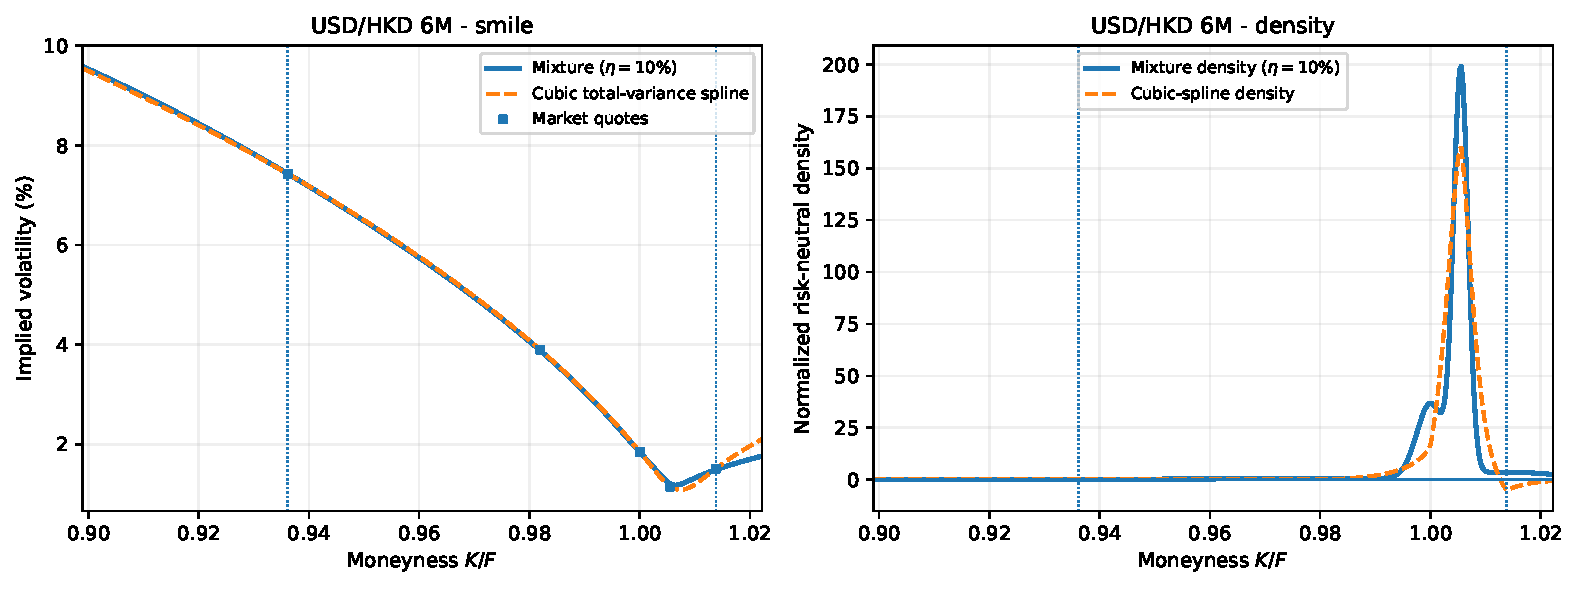
\includegraphics[width=0.98\textwidth]{fx_usdhkd_6mo.pdf}
\caption{USD/HKD 6M with $\eta=10\%$. The mixture remains density-positive on the plotted range. The cubic total-variance spline reproduces the knots exactly but develops a negative-density pocket outside the quoted region.}
\label{fig:usdhkd6m}
\end{figure}

\begin{figure}[H]
\centering
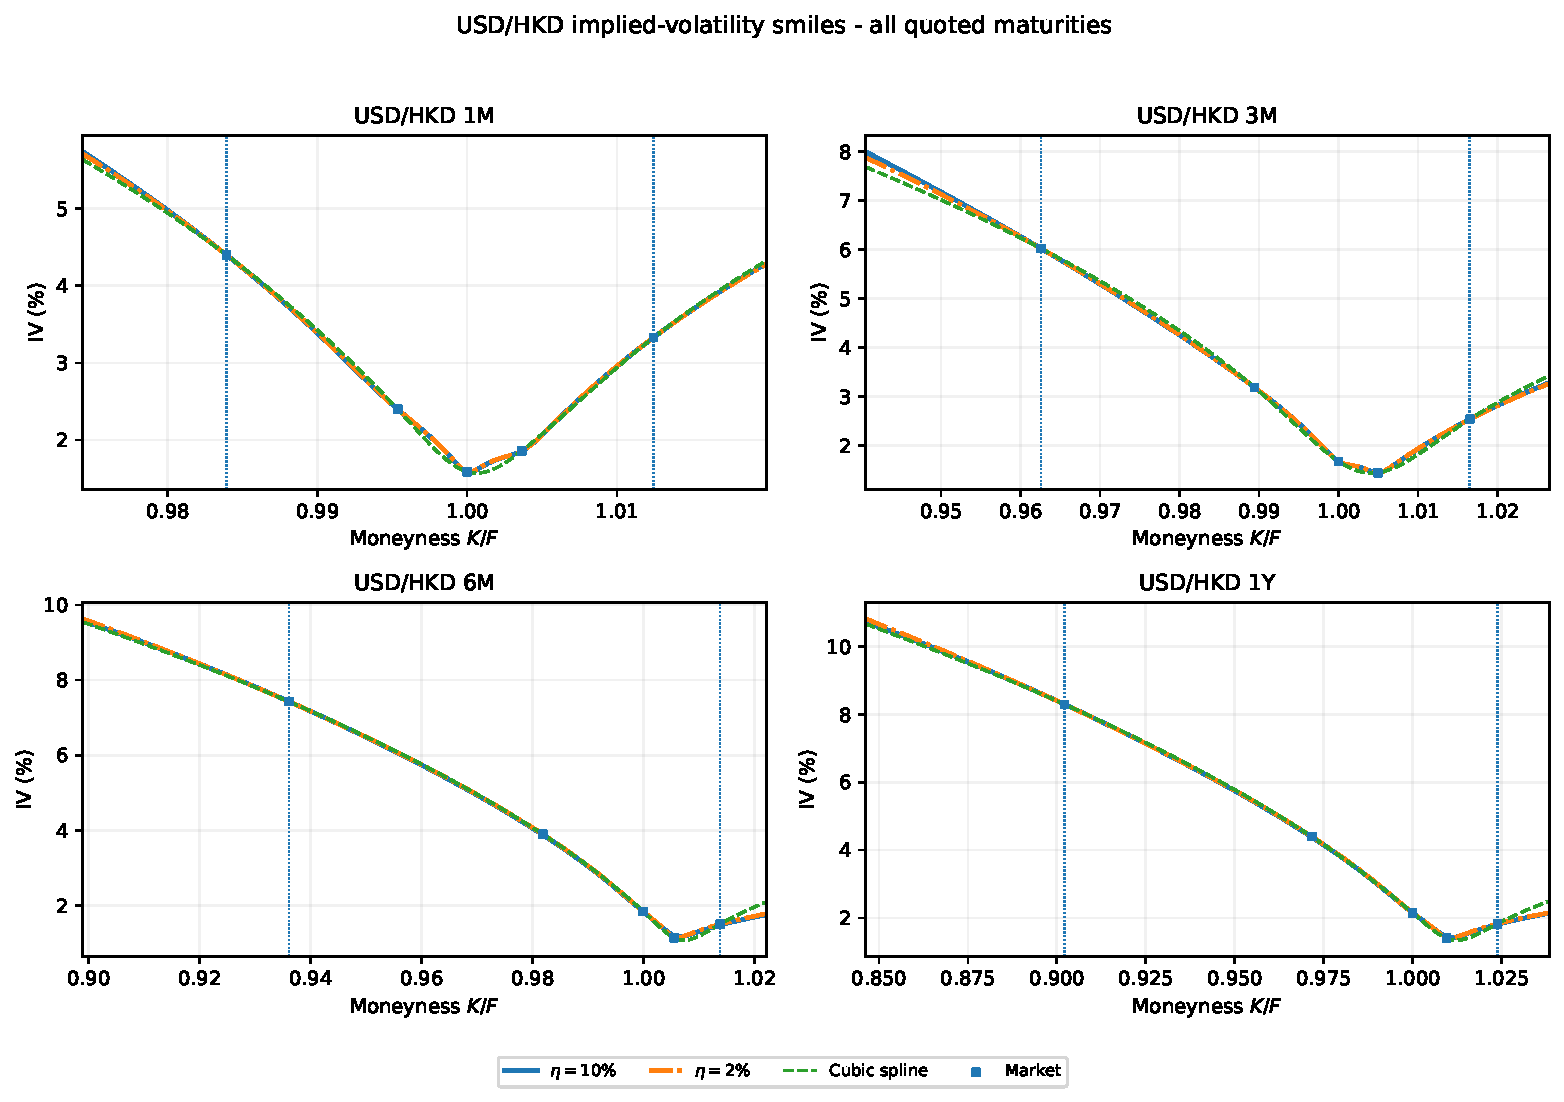
\includegraphics[width=0.98\textwidth]{fx_usdhkd_all_maturities_eta.pdf}
\caption{USD/HKD smiles at 1M, 3M, 6M, and 1Y. The 2\% floor is shown in addition to the 10\% floor. The difference is especially important for the strongly skewed 6M and 1Y smiles. Market quotes use small square markers.}
\label{fig:hkdallsmiles}
\end{figure}

\begin{figure}[H]
\centering
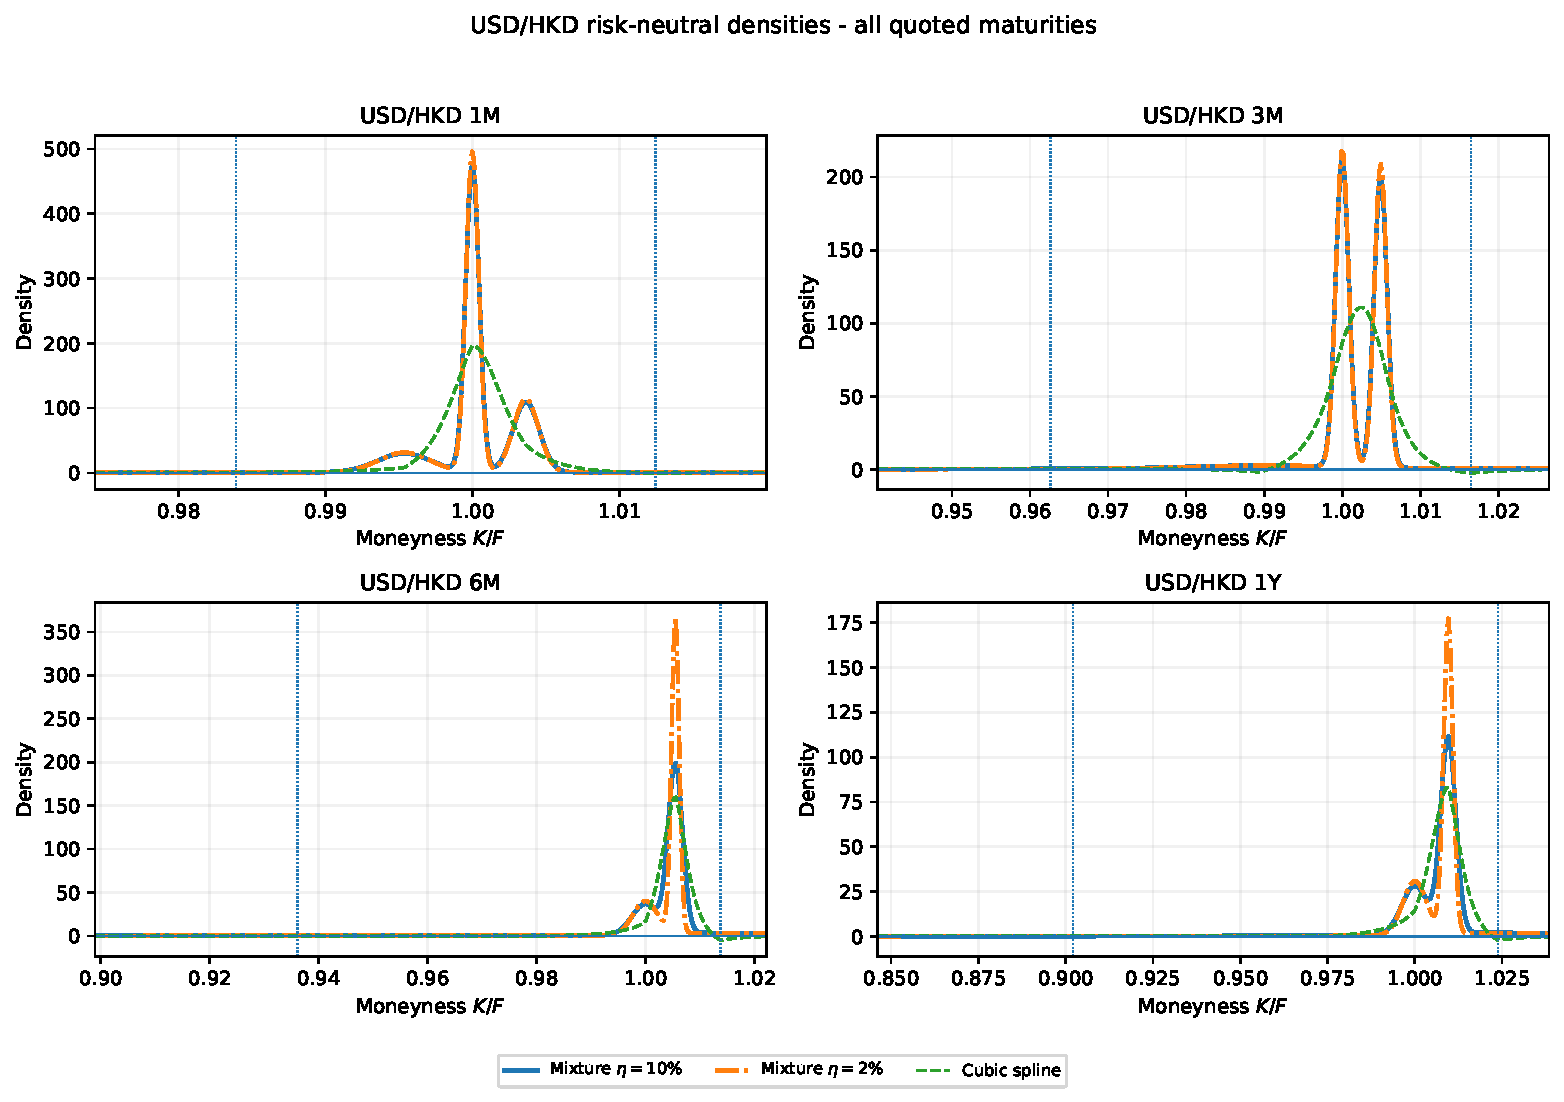
\includegraphics[width=0.98\textwidth]{fx_usdhkd_all_maturities_density_eta.pdf}
\caption{USD/HKD risk-neutral densities at all four quoted maturities. Both mixture calibrations remain positive on the displayed ranges, whereas the cubic total-variance interpolation may produce negative density between or beyond knots.}
\label{fig:hkdalldensities}
\end{figure}

\subsubsection*{Equity and equity-index market-region results}\label{sec:eqmarket}
The equity study uses dense grids: 30 SPY quotes, 30 TSLA quotes, 22 NVDA quotes, and 22 AAPL quotes for October 2026. We also use a 31-knot EURO STOXX 50 numerical benchmark obtained by an arbitrage-preserving densification of historical call quotes. The latter is therefore a numerical stress grid rather than 31 independent raw exchange observations.

This subsection deliberately reports the \emph{flat-kernel} mixture only. The right-wing modification is not used here; it is studied separately in Section~\ref{sec:wingresults}. This separation makes the market-region interpolation quality visible before any extrapolation control is introduced.

\begin{table}[H]
\centering
\caption{Dense equity/index market-region diagnostics using the flat-kernel mixture. The right-wing control is not used in this table.}
\label{tab:eqmarket}
\small
\resizebox{\textwidth}{!}{%
\begin{tabular}{lrrrrrr}
\toprule
Dataset & Quotes & Max IV err. 10\% (bp) & Max IV err. 2\% (bp) & Min. dens. 10\% & Min. dens. 2\% & Min. cubic dens. \\
\midrule
SPY, 2026-10-16  & 30 & 3.06 & 0.89 & $3.90\times10^{-5}$ & $2.90\times10^{-4}$ & -8.176 \\
TSLA, 2026-10-16 & 30 & 20.89 & 4.35 & 0.0220 & 0.0219 & -3.615 \\
NVDA, 2026-10-16 & 22 & 20.43 & 3.99 & $1.58\times10^{-8}$ & $7.09\times10^{-5}$ & -0.026 \\
AAPL, 2026-10-16 & 22 & 21.07 & 4.65 & 0.0217 & 0.0211 & -1.426 \\
EURO STOXX 50, 2014-10-17 & 31 & 25.53 & 20.93 & 0.0644 & 0.0631 & -16.589 \\
EURO STOXX 50, 2014-12-19 & 31 & 8.66 & 8.61 & 0.2968 & 0.3073 & -6.600 \\
EURO STOXX 50, 2015-03-20 & 31 & 6.00 & 9.42 & 0.2248 & 0.1527 & -4.106 \\
\bottomrule
\end{tabular}%
}
\end{table}

\begin{figure}[H]
\centering
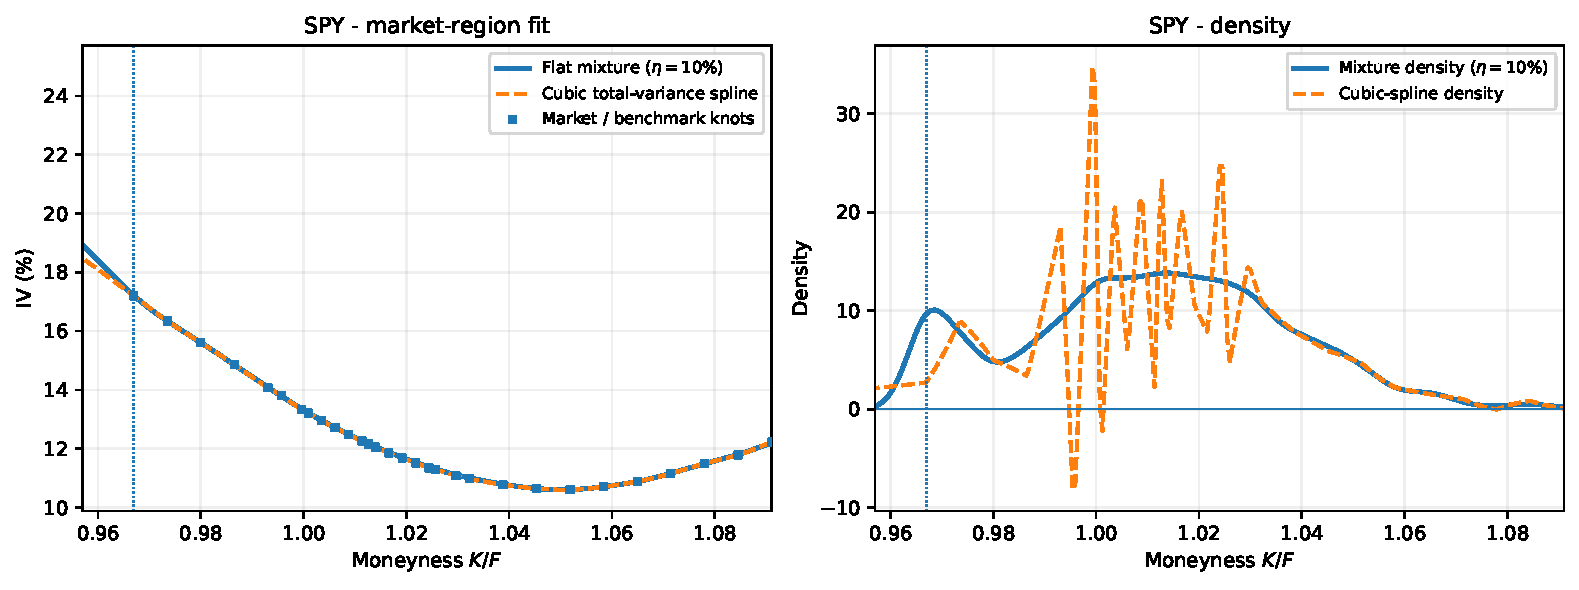
\includegraphics[width=0.98\textwidth]{equity_spy_flat.pdf}
\caption{SPY dense smile: flat-kernel mixture versus cubic total-variance interpolation. The plotting range stays close to the observed region so that knot-by-knot interpolation quality remains visible.}
\label{fig:spyflat}
\end{figure}

\begin{figure}[H]
\centering
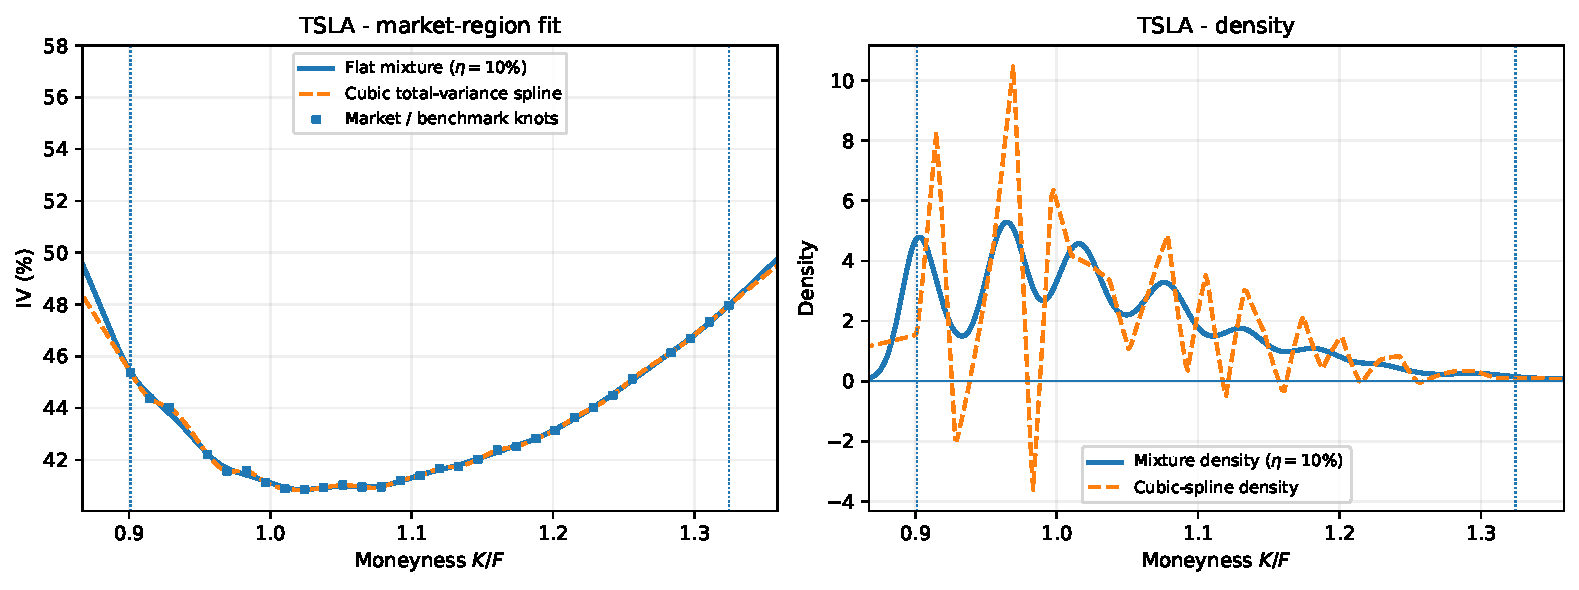
\includegraphics[width=0.98\textwidth]{equity_tsla_flat.pdf}
\caption{TSLA dense smile: flat-kernel mixture versus cubic total-variance interpolation. The cubic spline is exact at the knots, but its second derivative oscillates enough to create negative density between quotes.}
\label{fig:tslaflat}
\end{figure}

\begin{figure}[H]
\centering
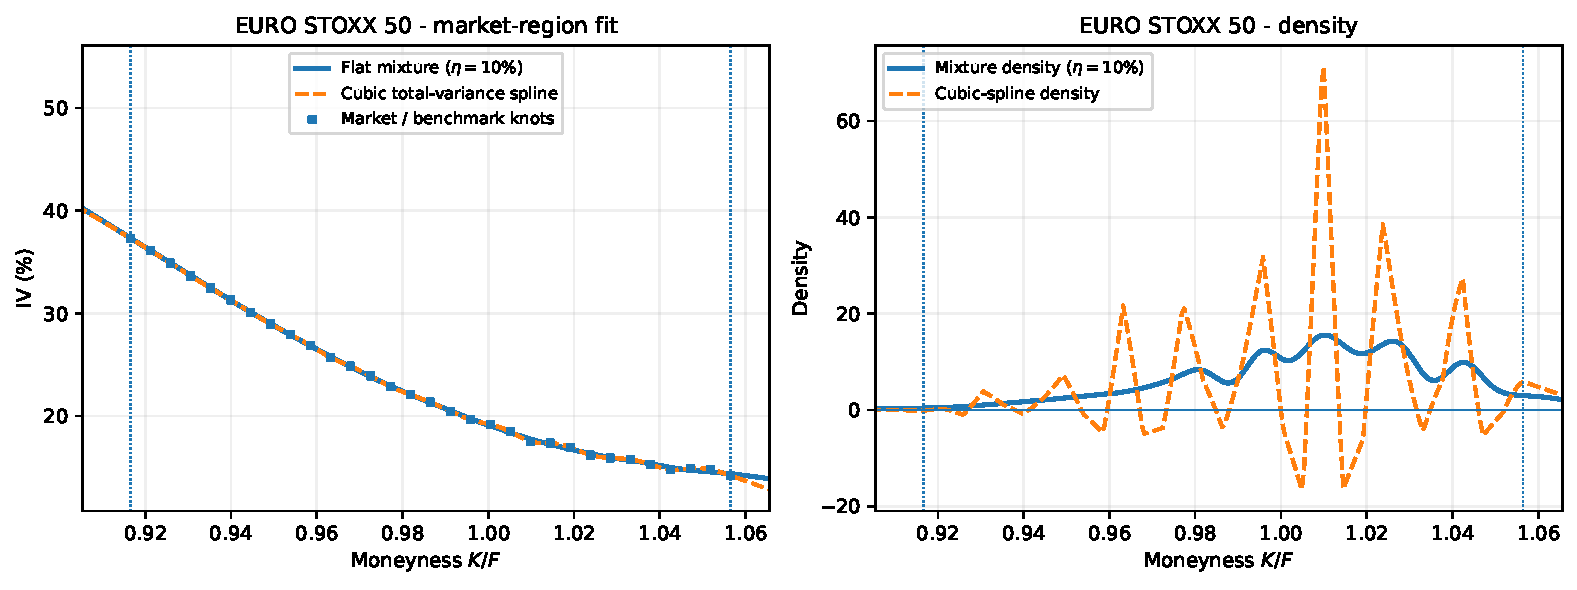
\includegraphics[width=0.98\textwidth]{equity_eurostoxx_flat.pdf}
\caption{EURO STOXX 50 31-knot benchmark. The dense grid is useful for assessing interpolation quality locally.}
\label{fig:euroflat}
\end{figure}

\begin{figure}[H]
\centering
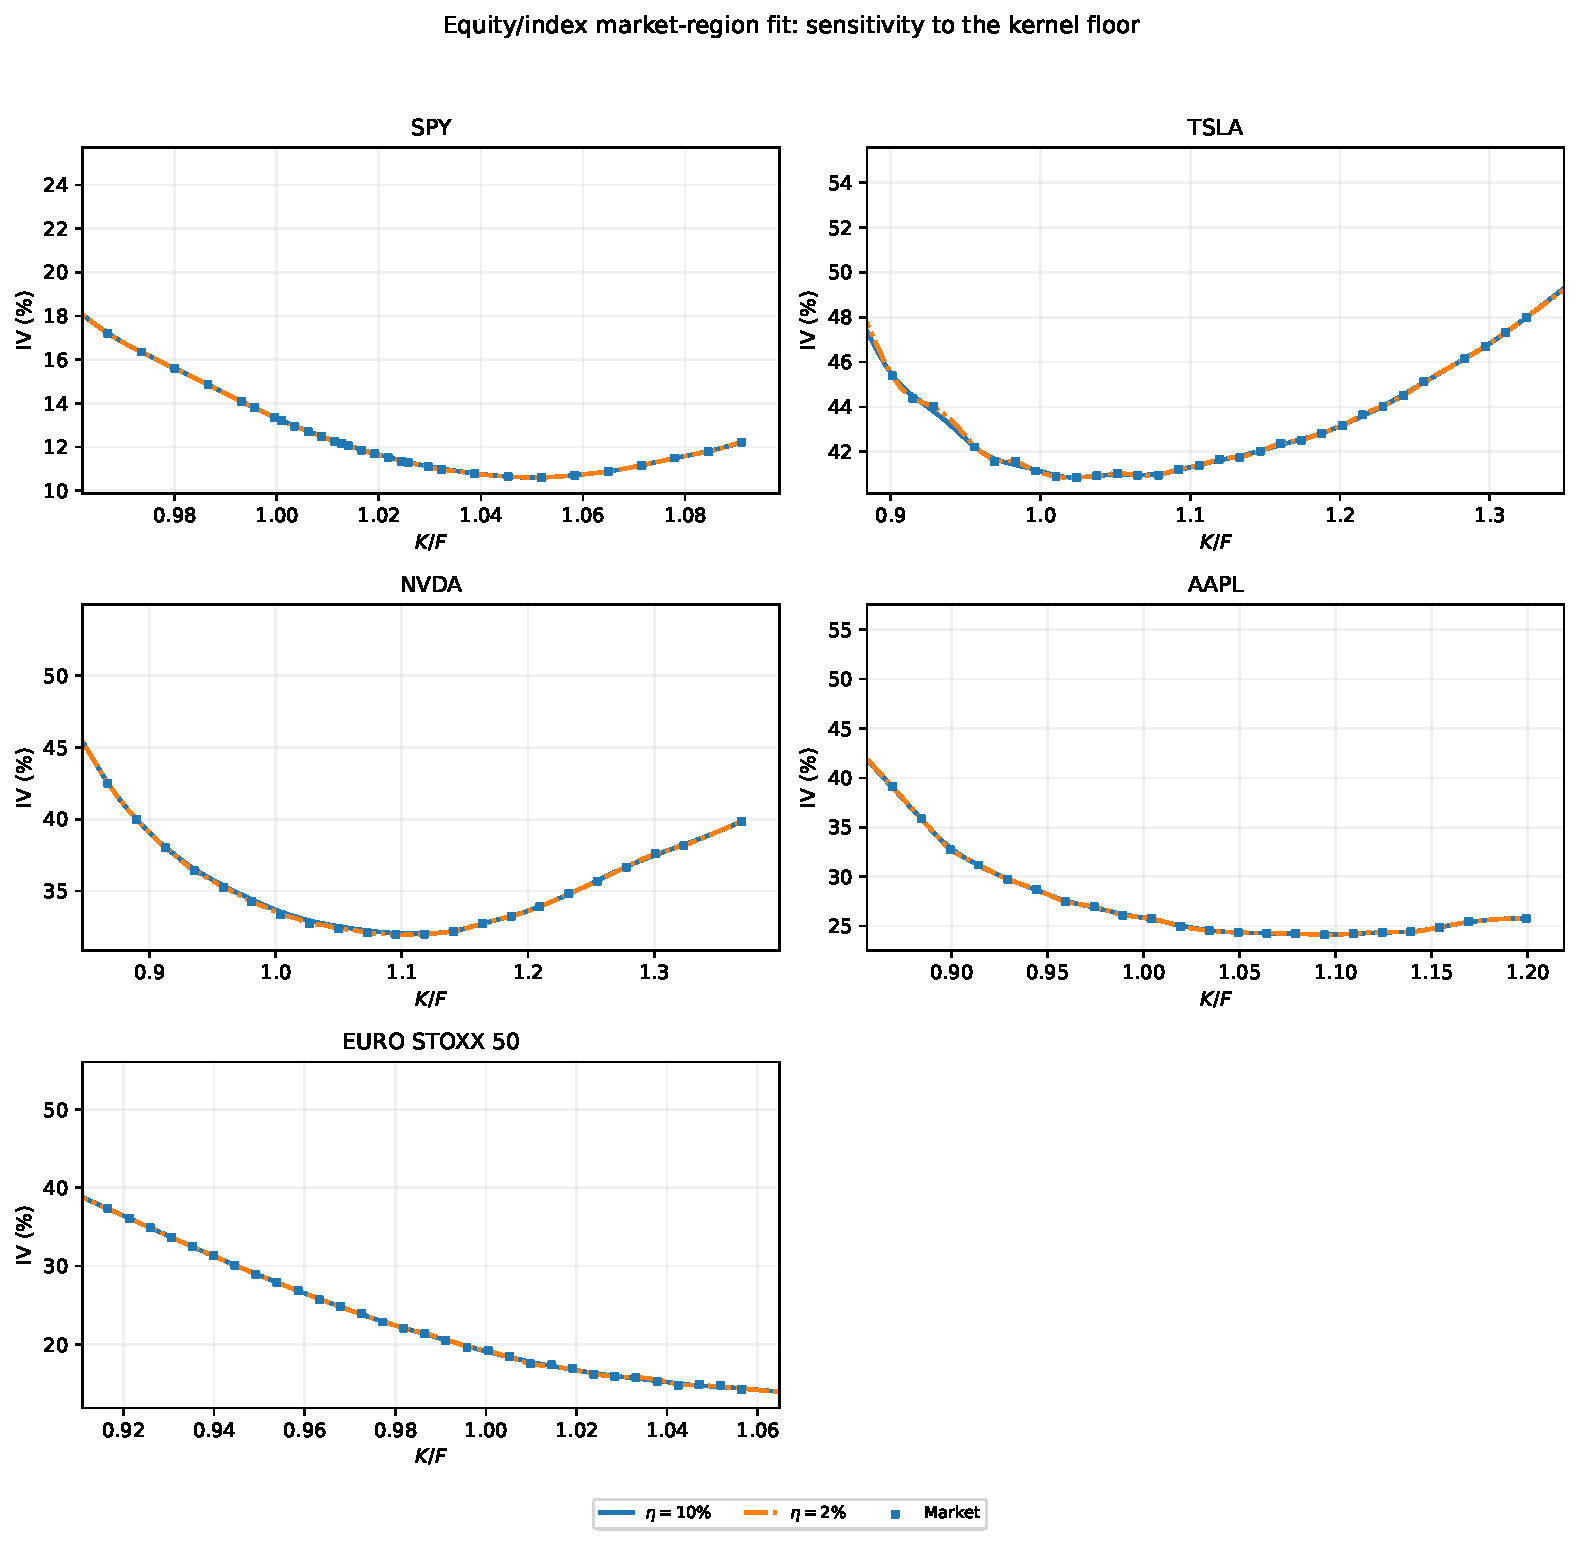
\includegraphics[width=0.98\textwidth]{equity_eta_smiles.pdf}
\caption{Sensitivity of dense equity/index fits to the lower kernel-width bound. The 2\% floor gives substantially more flexibility for SPY, TSLA, NVDA, and AAPL. The effect is less uniform on the densified EURO STOXX 50 stress grid. Market quotes are shown with small square markers.}
\label{fig:eqetasmile}
\end{figure}

\begin{figure}[H]
\centering
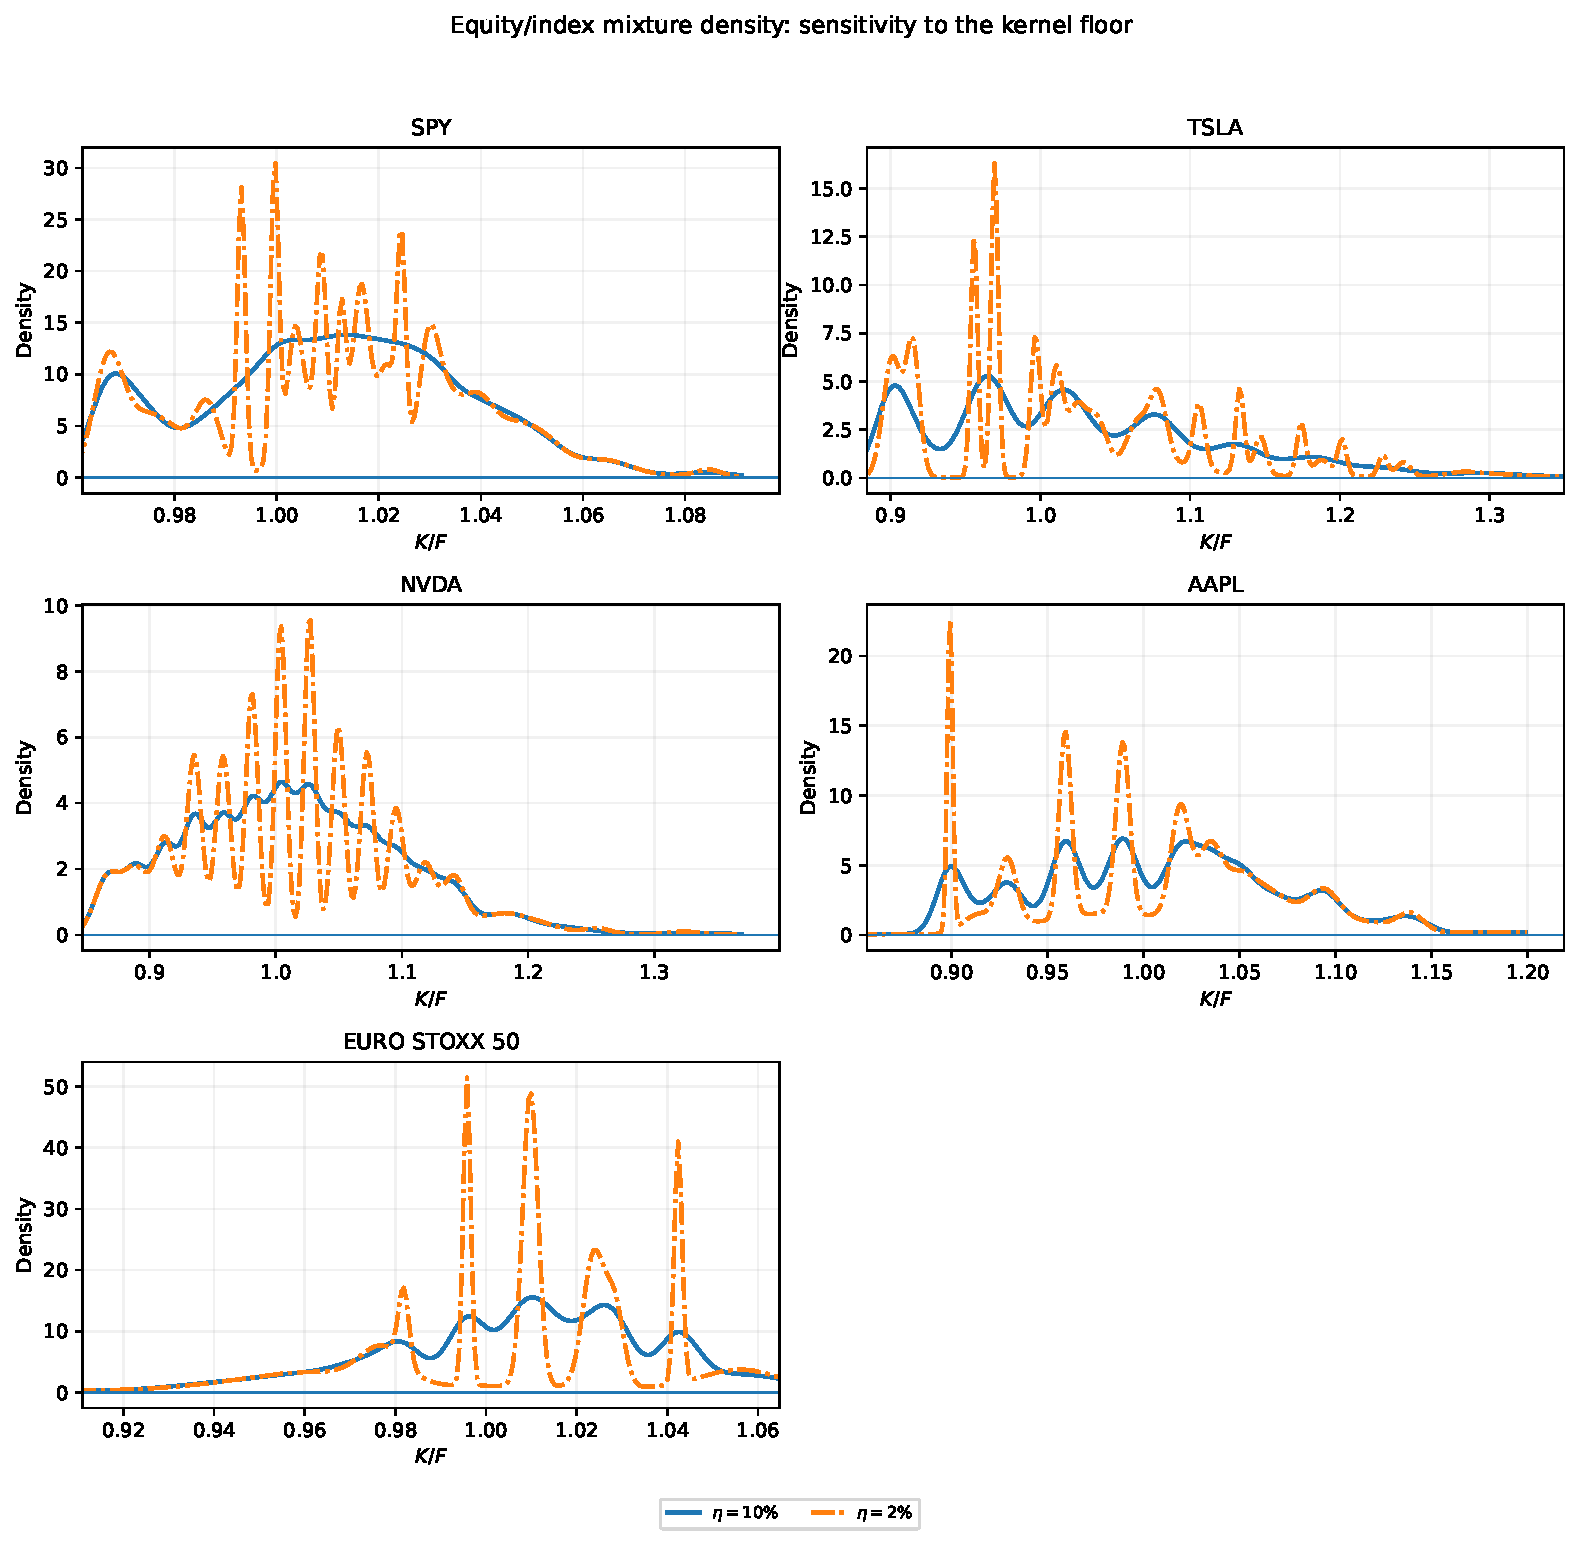
\includegraphics[width=0.98\textwidth]{equity_eta_densities.pdf}
\caption{Mixture-density sensitivity to $\eta$. Lowering the floor from 10\% to 2\% permits narrower kernels; this can improve the market fit but also changes local density concentration. Both curves remain non-negative on the displayed grids.}
\label{fig:eqetadensity}
\end{figure}

The main message of this section is that pointwise interpolation and density regularity are distinct objectives. A natural cubic spline of total variance may be visually smooth and exact at every quote while generating a highly oscillatory or negative density between knots. The log-normal mixture controls the density more directly, although practical lower and upper width restrictions can prevent an exact fit of every dense equity quote. The comparison of $\eta=10\%$ and $\eta=2\%$ makes this regularization trade-off explicit: the smaller floor often improves the fit, but it allows more localized kernels and is therefore not automatically preferable for every dataset.

\subsection{Equity volatility-wing extrapolation}\label{sec:wingresults}
The previous section intentionally kept the original flat-kernel extrapolation. We now isolate the extrapolation problem and compare that baseline with an equity-specific right-wing control. The comparison is performed only beyond the last observed market strike, so the fitted market region is unchanged.

Let
\[
x=\log(K/F),\qquad x_R=\log k_R
\]
where $k_R$ is the last observed market moneyness. For $x\le x_R$, every component keeps its calibrated width $\sigma_i^\star$. For $x>x_R$ we use
\begin{equation}
\sigma_i(x)=\sigma_i^\star
\exp\!\left[
-\alpha_R
\left(\frac{\sigma_i^\star}{\sigma_{\rm ATM}}\right)^2
(x-x_R)^2
\right].
\label{eq:controlledwing}
\end{equation}
Broad kernels are therefore damped more strongly than narrow kernels. The quadratic attachment makes the first derivative of each width vanish at $x_R$, avoiding a discontinuity in the fitted market smile.

Because the widths now depend on strike, positivity is no longer automatic merely from the original mixture formula. The parameter $\alpha_R$ is therefore selected numerically subject to direct checks of call monotonicity, call convexity, and non-negative density over the extrapolation grid. The target is the smallest admissible value that makes the aggregate right-wing implied volatility non-increasing after a short attachment region whenever such a value exists.

The figures below deliberately display much more of the \emph{right} extrapolation than the market-region plots. The flat-kernel curve is repeated only as a dashed reference so that the effect of the controlled wing can be seen directly.

\begin{table}[H]
\centering
\caption{Right-wing stress cases. Endpoint IVs refer to the far right edge of the plotted extrapolation grid.}
\label{tab:wings}
\begin{tabular}{lrrrr}
\toprule
Dataset & Last market IV & Flat-wing endpoint IV & Controlled endpoint IV & $\alpha_R$ \\
\midrule
SPX, 2026-07-31  & 17.66\% & 24.64\% & 10.31\% & 957.43 \\
TSLA, 2026-09-14 & 33.00\% & 41.65\% & 15.85\% & 264.53 \\
\bottomrule
\end{tabular}
\end{table}

\begin{figure}[H]
\centering
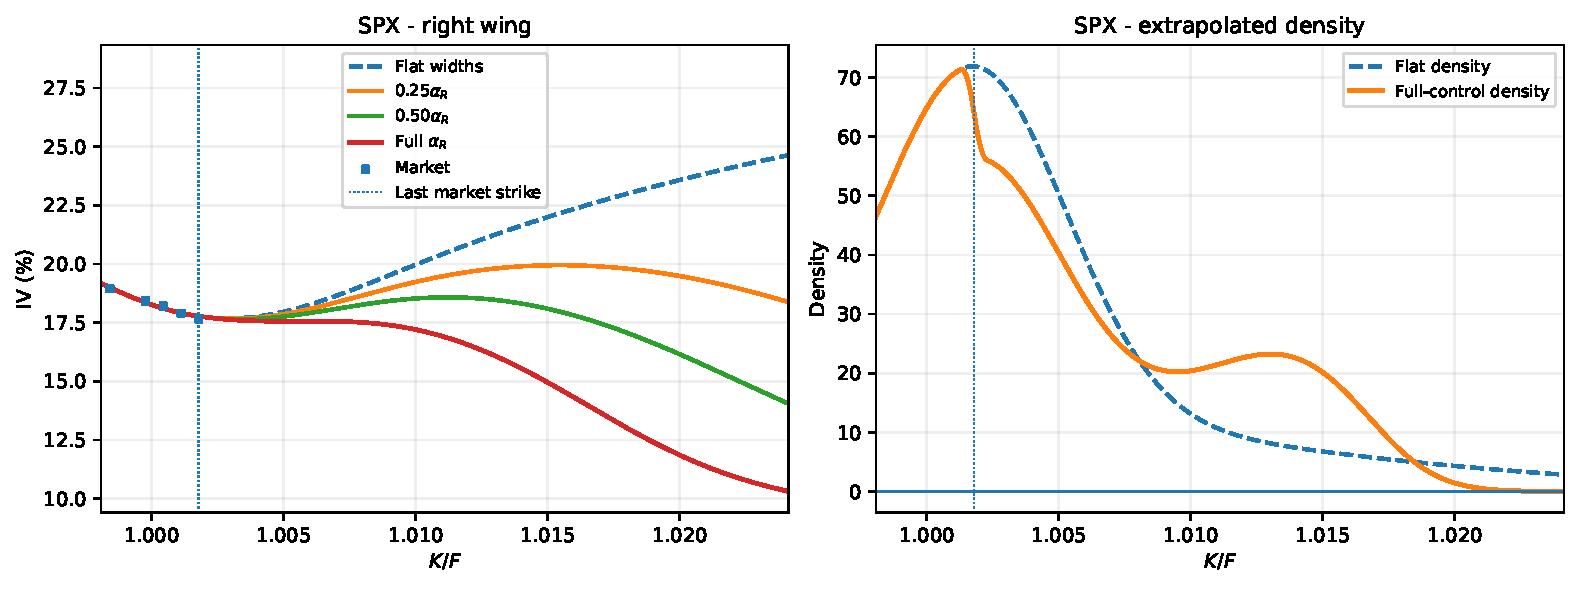
\includegraphics[width=0.98\textwidth]{wing_spx_stress.pdf}
\caption{SPX right-wing stress test. In addition to the flat-kernel extrapolation, the smile is shown for three strengths of the right-wing control: $0.25\alpha_R$, $0.50\alpha_R$, and the full $\alpha_R$. The milder controls reduce the unrealistic upward tail without forcing the strong decrease produced by the full control. Market quotes are shown with small square markers.}
\label{fig:spxwing}
\end{figure}

For SPX, the full monotonicity-target value of $\alpha_R$ is shown together with two milder alternatives. At the far-right endpoint of the displayed stress grid, the flat mixture gives approximately $24.64\%$ implied volatility, whereas the $0.25\alpha_R$, $0.50\alpha_R$, and full-control curves give approximately $18.38\%$, $14.05\%$, and $10.31\%$, respectively. This makes the wing parameter a transparent extrapolation choice rather than suggesting that the most aggressive admissible decay is necessarily the preferred market convention.

\begin{figure}[H]
\centering
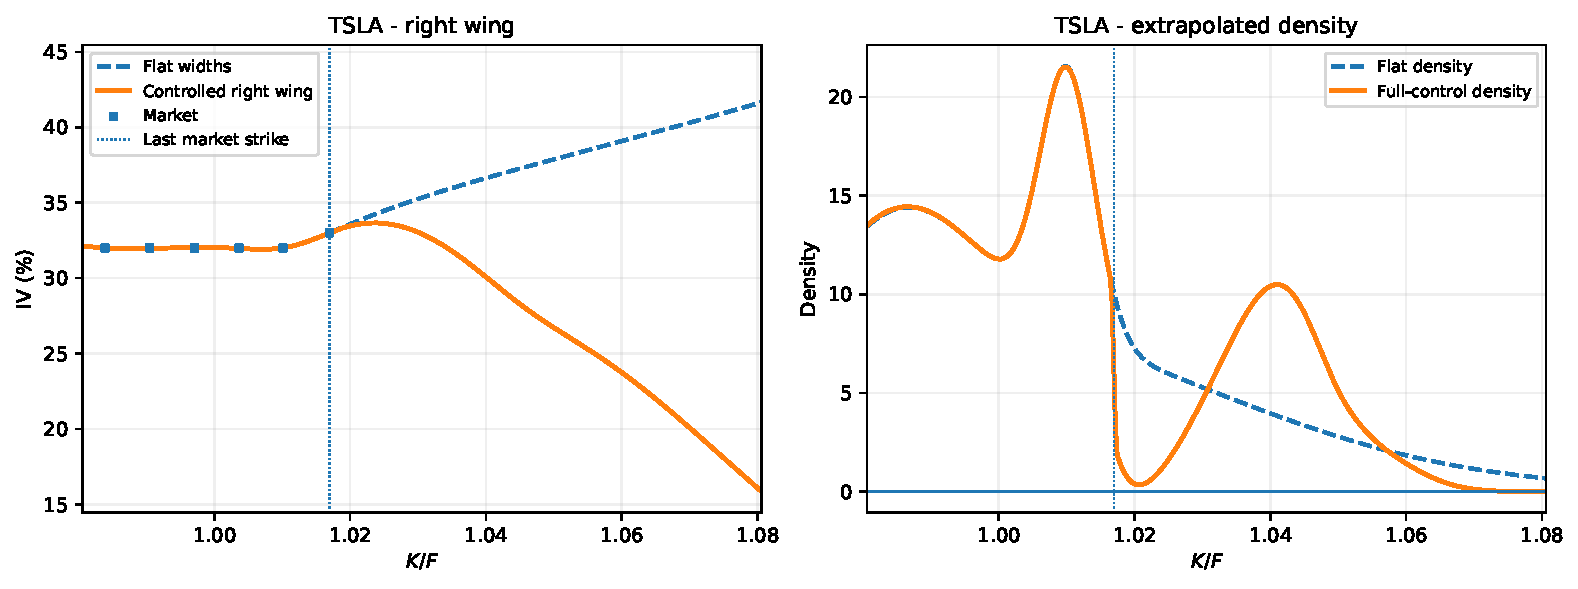
\includegraphics[width=0.98\textwidth]{wing_tsla_stress.pdf}
\caption{TSLA right-wing stress test. The flat-kernel extrapolation rises from the final market quote toward a much higher remote IV. The controlled wing reverses the long-run slope while the density remains non-negative on the tested grid. A small attachment shoulder can remain because the market's final local slope itself is not decreasing.}
\label{fig:tslawing}
\end{figure}

These tests illustrate why the extrapolation rule is treated separately from calibration. Inside the market, the original mixture parameters are retained. Outside the market, an equity-specific tail rule can be applied without changing any quoted call price. The numerical checks are part of the construction because strike-dependent kernel widths do not inherit the global positivity guarantee of a constant-width mixture automatically.

\section{Conclusion and future work}
In this paper, we have designed an arbitrage-free, efficient, and easily implementable construction of the volatility smile. We have shown that a perfect fit is possible whenever the market volatility quotes are arbitrage-free. The calibration produces smooth densities that can accommodate multi-modal distributions, particularly in pegged currencies. This representation also provides closed-form formulas for local volatility, the density, and European option prices, while remaining arbitrage-free and consistent with the market. Furthermore, the model may reveal clusters that are hidden in the quoted smile, such as those observed in the USD/HKD example.

This revised version preserves the theoretical construction of the original article \cite{elalaoui2023} and corrects the calendar-spread compact interval to $[\eta,k_{\max}]$. The numerical section now includes both $\eta=10\%$ and $\eta=2\%$, the four quoted USD/HKD maturities, and dense equity examples. For equities, the wing-control experiment is reported separately from the original flat-kernel calibration so that the extrapolation choice is clearly distinguished from the fitted market smile. The SPX experiment also shows several strengths of the wing-control parameter, illustrating that a milder decay may be preferable when the full monotonicity-target value decreases too aggressively. The reference to Cousot \cite{cousot2007} has been added in this revision because those related exact-calibration results were not known to the author when the previous version was written; the strike-wise linear interpolation used in the present construction remains distinct from Cousot's model construction.

In future work, it would be useful to study alternative analytic wing parametrizations and joint calibration across maturities while retaining the same arbitrage-free mixture construction.

\begin{thebibliography}{99}
\bibitem{blackscholes} F. Black and M. Scholes, ``The Pricing of Options and Corporate Liabilities,'' \emph{Journal of Political Economy}, 81, 637--654, 1973.
\bibitem{brigo2002} D. Brigo and F. Mercurio, ``Lognormal-Mixture Dynamics and Calibration to Market Volatility Smiles,'' \emph{International Journal of Theoretical and Applied Finance}, 5, 427--446, 2002.
\bibitem{brigo2000} D. Brigo and F. Mercurio, ``Analytical Models for Volatility Smiles and Skews,'' Banca IMI internal report, 2000.
\bibitem{mixedup} D. Brigo and F. Mercurio, ``A Mixed-Up Smile,'' \emph{Risk}, September 2000, 123--126.
\bibitem{cousot2007} L. Cousot, ``Conditions on Option Prices for Absence of Arbitrage and Exact Calibration,'' \emph{Journal of Banking \& Finance}, 31(11), 3377--3397, 2007, doi:10.1016/j.jbankfin.2007.04.006.
\bibitem{blacqueflorentin} P.-M. Blacque-Florentin and B. Missaoui, ``Nonparametric and Arbitrage-Free Construction of Call Surfaces Using $\ell^1$-Recovery.''
\bibitem{demarch} H. De March and P. Henry-Labord\`ere, ``Building Arbitrage-Free Implied Volatility: Sinkhorn's Algorithm and Variants,'' 2019.
\bibitem{andreasenhuge} J. Andreasen and B. Huge, ``Expanded Forward Volatility,'' \emph{Risk}, 26(1), 101--107, 2013.
\bibitem{liptonsepp} A. Lipton and A. Sepp, ``Filling the Gaps,'' 2011.
\bibitem{dupire1997} B. Dupire, ``Pricing and Hedging with Smiles,'' in \emph{Mathematics of Derivative Securities}, 1997.
\bibitem{dupire1994} B. Dupire, ``Pricing with a Smile,'' \emph{Risk}, 1994.
\bibitem{poincare} H. Poincar\'e, ``Sur certaines solutions particuli\`eres du probl\`eme des trois corps,'' \emph{C. R. Acad. Sci. Paris}, 97, 251--252, 1883.
\bibitem{blochcoello} D. A. Bloch and C. C. Coello, ``Smiling at Evolution,'' \emph{Applied Soft Computing}, 11(8), 5724--5734, 2011.
\bibitem{kahale} N. Kahal\'e, ``An Arbitrage-Free Interpolation of Volatilities,'' \emph{Risk}, 17, 102--106, 2004.
\bibitem{gatheraljacquier} J. Gatheral and A. Jacquier, ``Arbitrage-Free SVI Volatility Surfaces,'' \emph{Quantitative Finance}, 14(1), 59--71, 2014.
\bibitem{fengler} M. Fengler, ``Arbitrage-Free Smoothing of the Implied Volatility Surface,'' \emph{Quantitative Finance}, 9(4), 417--428, 2009.
\bibitem{clark} I. J. Clark, \emph{Foreign Exchange Option Pricing: A Practitioner's Guide}, Wiley, 2011.
\bibitem{elalaoui2023} A. El Alaoui, ``Volatility Surfaces and Log-Normal Mixture: Crafting an Arbitrage-Free Calibration,'' SSRN Working Paper 4602237, 2023; revised 2025, doi:10.2139/ssrn.4602237.
\bibitem{bofa2025} BofA Global Research, \emph{The EM Asia FX Strategist}, 21 May 2025, Exhibits 22--25 (USD/HKD implied-volatility surface and smiles).
\end{thebibliography}

\end{document}
